\documentclass[answers]{exam}
\usepackage{texPreamble}
\usepackage{relsize}
\usepackage{tabularx}
\extraheadheight{0.25in}
\extrafootheight{1.0in}
\extrawidth{1in}
% ----------------------------------------------------------------
\firstpagefootrule
\runningfootrule
\begin{document}
%\relscale{1.4}
\section{4.3: What Derivatives Tell Us}
\begin{defn*}[Increasing and Decreasing Functions]
  Suppose a function $f$ is defined on an interval $I$. We say that $f$ is increasing on $I$ if $f(x_2)>f(x_1)$ whenever $x_1$ and $x_2$ are in $I$ and $x_2>x_1$. We say that $f$ is decreasing on $I$ if $f(x_2)<f(x_1)$ whenever $x_1$ and $x_2$ are in $I$ and $x_2>x_1$.
\end{defn*}
\begin{center}
  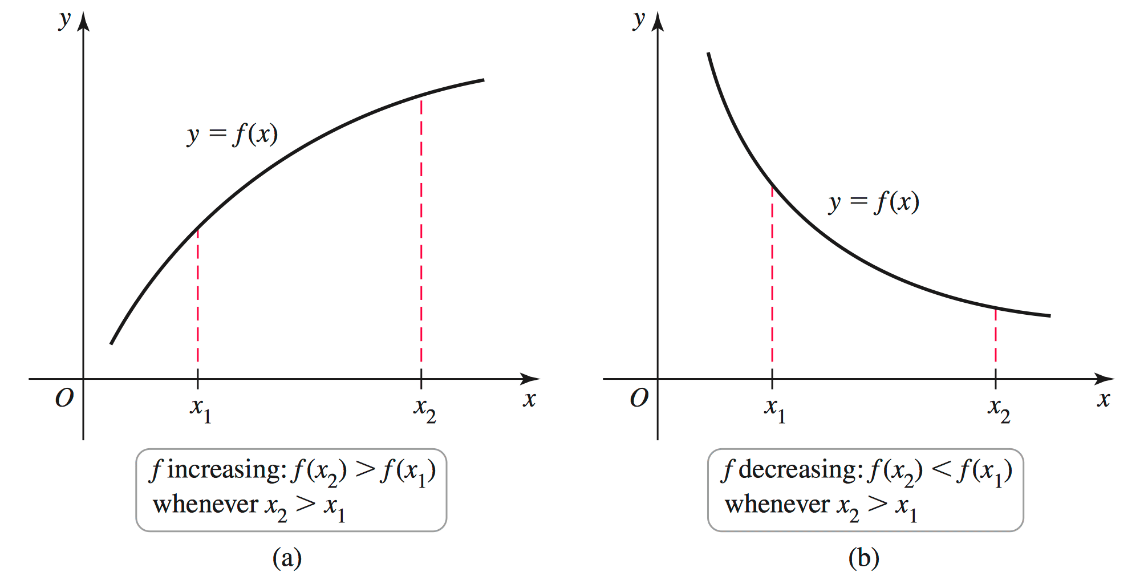
\includegraphics[width=0.65\linewidth]{images/briggs_04_03/fig4_20.png}
\end{center}

\vspace*{\stretch{1}}
\noindent
\fbox{\parbox{0.9875\linewidth}{
  \textbf{Theorem 4.7: Test for Intervals of Increase and Decrease}
  
  Suppose $f$ is continuous on an interval $I$ and differentiable at every interior point of $I$. If $f'(x)>0$ at all interior points of $I$, then $f$ is increasing on $I$. If $f'(x)<0$ at all interior points of $I$, then $f$ is decreasing on $I$.
}}
\begin{center}
  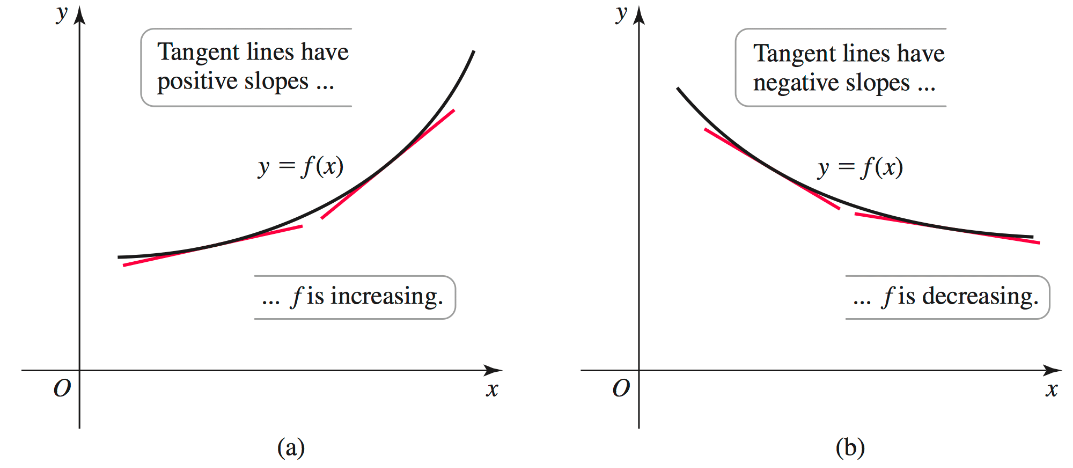
\includegraphics[width=0.65\linewidth]{images/briggs_04_03/fig4_21.png}
\end{center}
\pagebreak
\begin{proof}
  \textbf{(Theorem 4.7: Test for Intervals of Increase and Decrease) p258}

  Let $a$ and $b$ be any two distinct points in the interval $I$ with $b>a$. By the Mean Value Theorem, 
    $$\frac{f(b)-f(a)}{b-a}=f'(c)$$
  for some $c$ between $a$ and $b$. Equivalently,
    $$f(b)-f(a)=f'(c)(b-a).$$
  Notice that $b-a>0$ by assumption. So if $f'(c)>0$, then $f(b)-f(a)>0$. Therefore, for all $a$ and $b$ in $I$ with $b>a$, we have $f(b)>f(a)$, which implies that $f$ is increasing on $I$. Similarly, if $f'(c)<0$, then $f(b)-f(a)<0$ or $f(b)<f(a)$. It follows that $f$ is decreasing on $I$.
\end{proof}
\vspace*{\stretch{1}}

\noindent
\fbox{\parbox{0.9875\linewidth}{
  \textbf{Theorem 4.8: First Derivative Test}
  
  Assume that $f$ is continuous on an interval that contains a critical point $c$ and assume $f$ is differentiable on an interval containing $c$, except perhaps at $c$ itself.

\vspace*{10pt}
  \begin{minipage}{0.85\linewidth}
    \begin{itemize}
      \item If $f'$ changes sign from positive to negative as $x$ increases through $c$, then $f$ has a local maximum at $c$.
      \item If $f'$ changes sign from negative to positive as $x$ increases through $c$, then $f$ has a local minimum at $c$.
      \item If $f'$ does not change sign at $c$ (from positive to negative or vice versa), then $f$ has no local extreme value at $c$.
    \end{itemize}
  \end{minipage}
}}

\begin{center}
  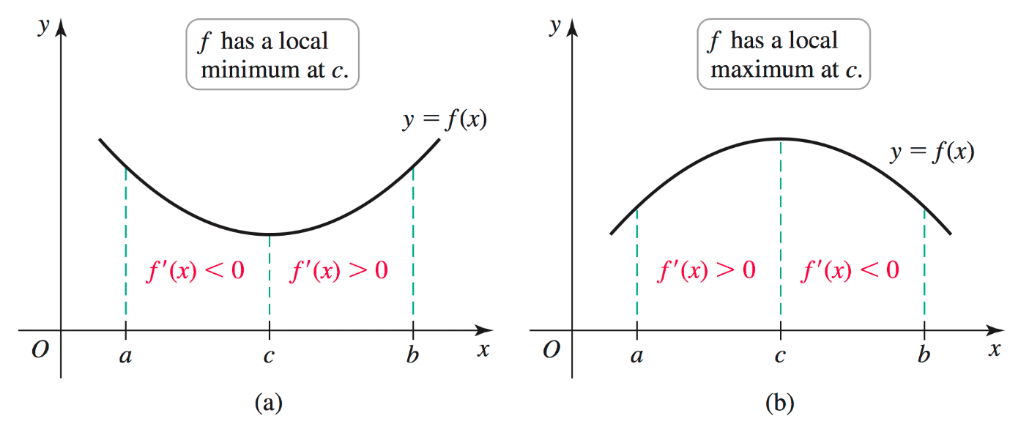
\includegraphics[width=0.65\linewidth]{images/briggs_04_03/fig4_26.png}
\end{center}
\vspace*{-35pt}
\pagebreak

\begin{ex*}
  Consider the function $f(x)=6x-x^3$.
\end{ex*}
  \begin{enumerate}[label=\alph*)]
    \item $f'(x)=$ \\[15pt]
    \item Find the intervals on which the function is increasing and decreasing.
      \setlength\itemsep{\stretch{1}}
    \item Identify the function's local extreme values, if any. (e.g. ``local max of \underline{\hspace*{15pt}} at $x=\underline{\hspace*{15pt}}$'')
    \item Which, if any, of the extreme values are absolute? 
  \end{enumerate}
\vspace*{\stretch{1}}
\pagebreak
\begin{ex*}
  Consider the function $f(t)=12t-t^3$ on $-3\leq t<\infty$.
\end{ex*}
\begin{enumerate}[label=\alph*)]
  \item $f'(t)=$ \\[15pt]
  \item Find the intervals on which the function is increasing and decreasing.
    \setlength\itemsep{\stretch{1}}
  \item Identify the function's local extreme values, if any. (e.g. ``local max of \underline{\hspace*{15pt}} at $x=\underline{\hspace*{15pt}}$'')
  \item Which, if any, of the extreme values are absolute? 
\end{enumerate}
\vspace*{\stretch{1}}
\pagebreak

\begin{ex*}
  Consider the function $f(x)=\cos^2(x)$ on $\sbrkt{-\pi,\pi}$. Find the intervals on which $f$ is increasing and the intervals on which it is decreasing.
\end{ex*}
\vspace*{\stretch{1}}
\pagebreak
\begin{defn*}[Concavity and Inflection Point]
  Let $f$ be differentiable on an open interval $I$. 
  \begin{itemize}
    \item If $f'$ is increasing on $I$, then $f$ is \textit{concave up} on $I$.
   
    \item If $f'$ is decreasing on $I$, then $f$ is \textit{concave down} on $I$.
  
  	\item If $f$ is continuous at $c$ and $f$ changes concavity at $c$, then $f$ has an \textit{inflection point} at $c$.
  \end{itemize}
\end{defn*}

\vspace*{\stretch{1}}
\begin{center}
  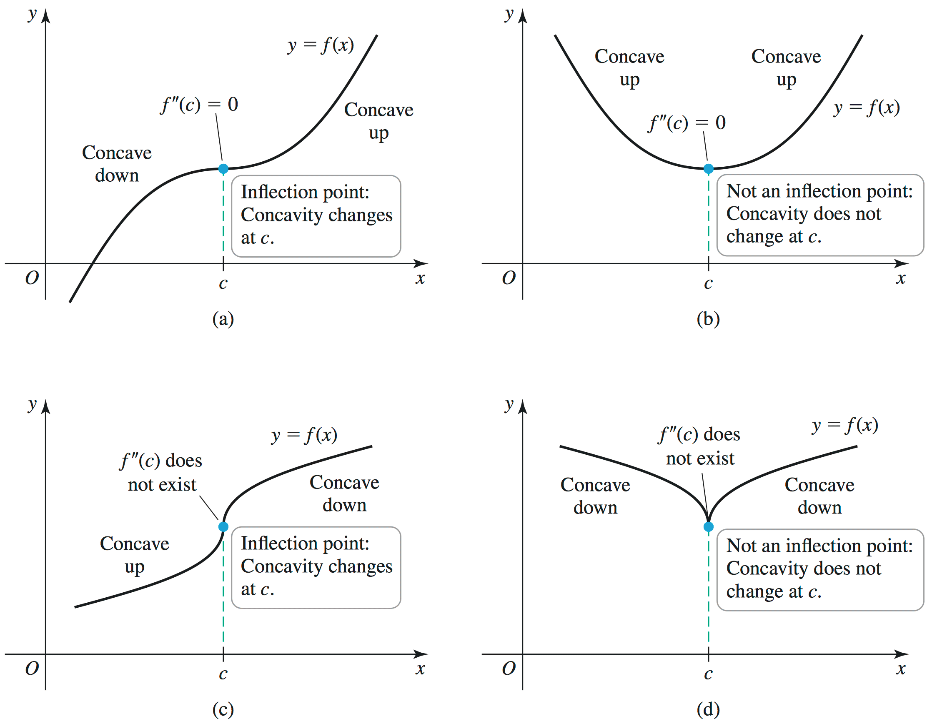
\includegraphics[width=0.925\linewidth]{images/briggs_04_03/fig4_35.png}
\end{center}
\pagebreak

\noindent
\fbox{\parbox{0.9875\linewidth}{
  \textbf{Theorem 4.10: Test for Concavity}
  
  Suppose $f''$ exists on an open interval $I$.
  \begin{itemize}
    \item If $f''>0$ on $I$, then $f$ is concave up on $I$.
    \item If $f''<0$ on $I$, then $f$ is concave down on $I$.
    \item If $c$ is a point of $I$ at which $f''$ changes sign at $c$, then $f$ has an inflection point at $c$.
  \end{itemize}
}}
\begin{ex*}
  Consider $f(x)=5-3x^2+x^3$
\end{ex*}
\begin{enumerate}[itemsep=\stretch{1}, label=\alph*)]
  \item Find the intervals of increasing/decreasing and local max/min.
  \item Find intervals of concavity and inflection points.
  \item Draw a rough sketch of the function.
\end{enumerate}
\vspace*{\stretch{1}}
\pagebreak

\begin{ex*}
  Consider $f(x)=xe\inv[x^2/2]$
\end{ex*}
\begin{enumerate}[itemsep=\stretch{1}, label=\alph*)]
  \item Find the intervals of increasing/decreasing and local max/min.
  \item Find intervals of concavity and inflection points.
  \item Draw a rough sketch of the function.
\end{enumerate}
\vspace*{\stretch{1}}
\pagebreak

\begin{ex*}
  Consider $f(x)=x\,\sqrt[3]{(x-3)^2}$
\end{ex*}
\begin{enumerate}[itemsep=\stretch{1}, label=\alph*)]
  \item Find the intervals of increasing/decreasing and local max/min.
  \item Find intervals of concavity and inflection points.
  \item Draw a rough sketch of the function.
\end{enumerate}
\vspace*{\stretch{1}}
\pagebreak

\begin{ex*}
  Consider $f(x)=x^2-x-\ln(x)$
\end{ex*}
\begin{enumerate}[itemsep=\stretch{1}, label=\alph*)]
  \item Find the intervals of increasing/decreasing and local max/min.
  \item Find intervals of concavity and inflection points.
  \item Draw a rough sketch of the function.
\end{enumerate}
\vspace*{\stretch{1}}
\pagebreak

\begin{ex*}
  Given the first derivative $y'=\parens{x-2}\inv[1/3]$
\end{ex*}
\begin{enumerate}[itemsep=\stretch{1}, label=\alph*)]
  \item Find the intervals of increasing/decreasing and local max/min of $y$.
  \item Find intervals of concavity and inflection points.
  \item Draw a rough sketch of the function.
\end{enumerate}
\vspace*{\stretch{1}}
\pagebreak

As a visual summary, here is figure 4.27 from Briggs:
\begin{center}
  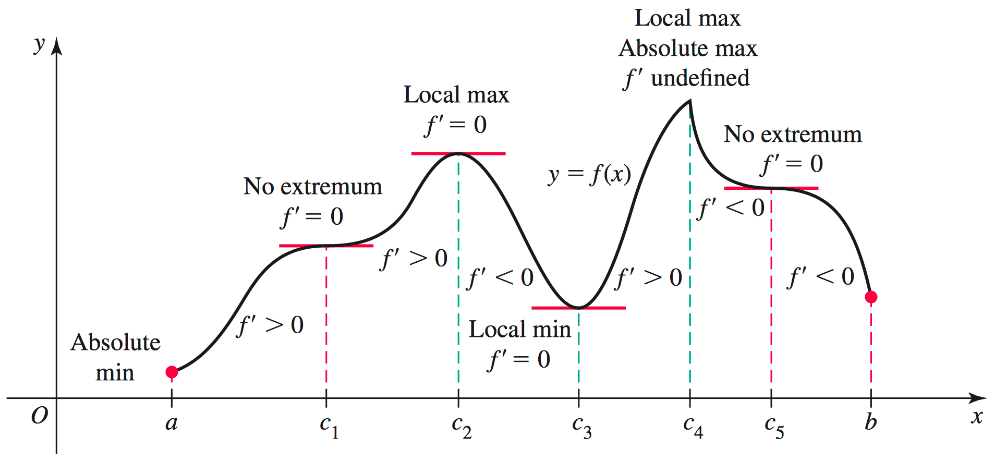
\includegraphics[width=0.85\linewidth]{images/briggs_04_03/fig4_27.png}
\end{center}
\vspace*{\stretch{1}}
\begin{center}
  \begin{tabularx}{0.95\linewidth}{*{3}{X}}\toprule
    $f(x)$& $f'(x)$& $f''(x)$\\\midrule
    increasing& positive& ---\\
    decreasing& negative& ---\\
    max& zero (pos to neg)& ---\\
    min& zero (neg to pos)& ---\\
    concave up& increasing& positive\\
    concave down& decreasing& negative\\
    Inflection point& max/min& changes sign\\\bottomrule
  \end{tabularx}
\end{center}
\vspace*{\stretch{1}}
\pagebreak

\noindent
\fbox{\parbox{0.9875\linewidth}{
  \textbf{Theorem 4.11: Second Derivative Test for Local Extrema}
  
  Suppose $f''$ is continuous on an open interval containing c with f'(c)=0.
  \begin{itemize}
    \item If $f''(c)>0$, then $f$ has a local minimum at $c$ (Figure 4.40a).
    \item If $f''(c)<0$, then $f$ has a local maximum at $c$  (Figure 4.40b).
    \item If $f''(c)=0$, then the test is inconclusive; $f$ may have a local maximum, local minimum, or neither at $c$.
  \end{itemize}
}}

\begin{center}
  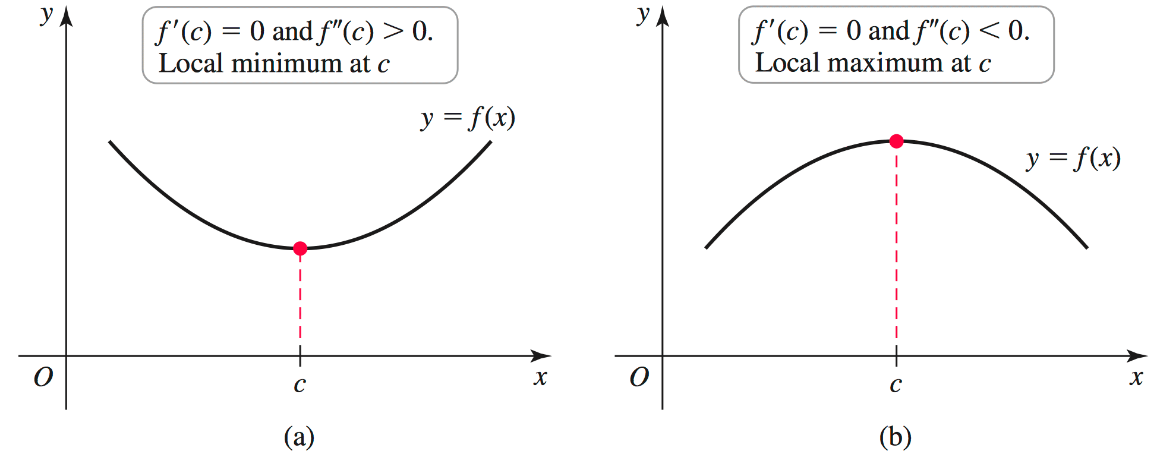
\includegraphics[width=0.8\linewidth]{images/briggs_04_03/fig4_40.png}
\end{center}
\begin{ex*}
  For each of the following, use the Second Derivative Test for Extrema to determine local max/mins:
\end{ex*}
\begin{tasks}(3)
  \task $f(x)=x^5-5x+3$
  \task $f(x)=2x^3-3x^2+12$
  \task $f(x)=x^3-6$
\end{tasks}
\pagebreak
\vspace*{\stretch{1}}
\begin{center}
  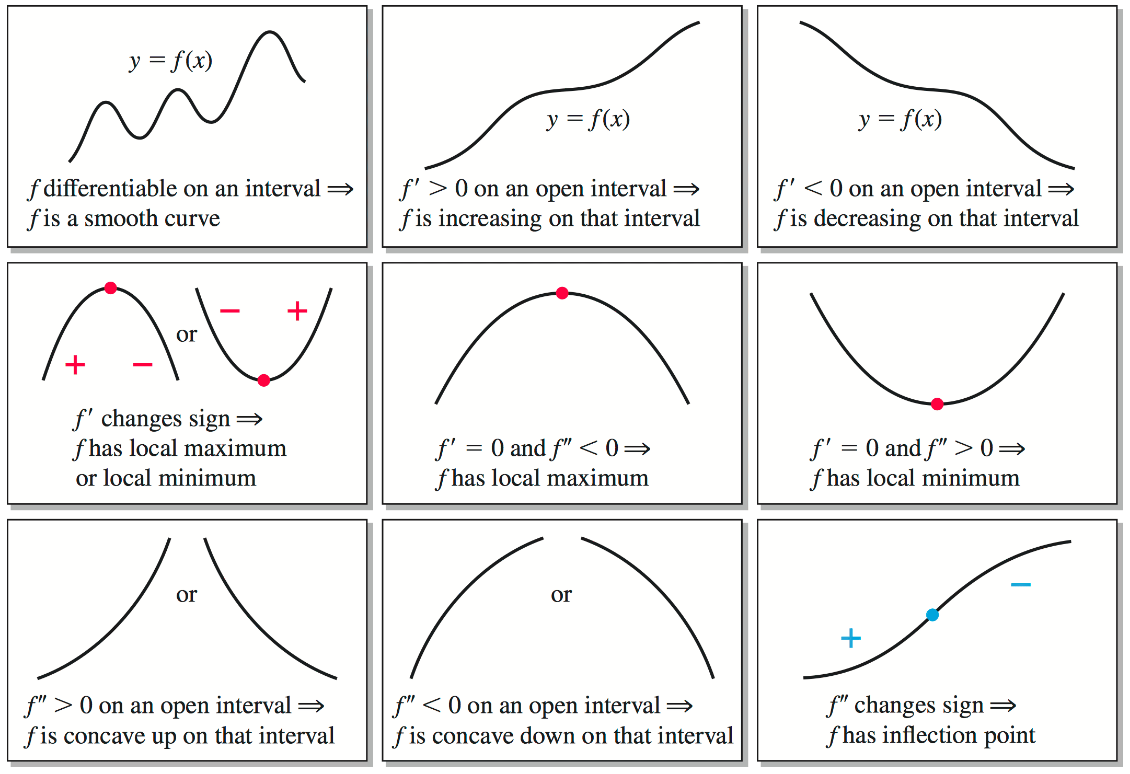
\includegraphics[width=1.0\linewidth]{images/briggs_04_03/fig4_43.png}
\end{center}
\vspace*{\stretch{1}}
\pagebreak

\end{document}
